% !TEX root = ../report.tex

\chapter{Експериментальний аналіз результатів та оцінка ефективності системи}
    \label{chap:results}

    У цьому розділі наводяться результати комплексного тестування розробленої моделі B-Mamba та її порівняльний аналіз із передовими архітектурами в галузі колоризації зображень.
    Дослідження ефективності проведено як за допомогою об'єктивних математичних метрик $\mathrm{PSNR}$, $\mathrm{SSIM}$ та $\mathrm{MSE}$,
    так і за допомогою перцептивних генеративних критеріїв $\mathrm{FID}$, $\mathrm{KID}$ та $\mathrm{LPIPS}$. 

    Окрім аналізу якості генерованого зображення, особлива увага приділяється апаратній ефективності запропонованого методу -- споживанню $\mathrm{VRAM}$ та кількості $\mathrm{Time}$,
    що є критично важливими параметрами для систем інтерактивного розфарбовування реального часу.

    \section{Апаратне забезпечення та параметри навчання}
        Процес навчання моделі здійснювався з використанням відеокарти NVIDIA GeForce RTX 5060 Ti та процесора AMD Ryzen 5 5600.
        Для забезпечення стабільності обчислень усі вхідні зображення масштабувалися до розміру $256 \times 256$ пікселів, а розмір пакету (англ. batch size) становив 16 екземплярів.
        
        Оптимізація вагових коефіцієнтів виконувалася за допомогою алгоритму AdamW із базовою швидкістю навчання $1 \times 10^{-4}$ та коефіцієнтом згасання ваг (англ. weight decay) $1 \times 10^{-4}$.
        Для динамічного адаптивного керування кроком оптимізації застосовувався планувальник CosineAnnealingLR із мінімальною швидкістю навчання $\eta_{\min} = 1 \times 10^{-6}$
        та тривалістю циклу, що відповідає загальній кількості епох навчання.
        
        Модель навчалася протягом 43 епох на тренувальній вибірці COCO 2017 Train, а валідація проводилася на COCO 2017 Val.
        Для розрахунку загальної цільової функції втрат було емпірично підібрано такі вагові коефіцієнти: $\lambda_{\mathrm{L1}} = 1.0$, $\lambda_{\mathrm{hint}} = 5.0$ та $\lambda_{\mathrm{LPIPS}} = 1.0$. 
        
        Для прискорення навчання та зменшення споживання відеопам'яті застосовувалася змішана точність обчислень у форматі BFloat16 (англ. Brain Floating Point 16).
        На відміну від стандартного Float32, цей формат майже вдвічі скорочує обсяг пам'яті, необхідний для зберігання проміжних активацій, тоді як основні вагові коефіцієнти зберігаються у форматі Float32 для чисельної стабільності градієнтного спуску. Завдяки цьому тривалість однієї епохи скоротилася приблизно з 90 до 60 хвилин.

        За підсумками процесу навчання значення функції втрат на тренувальній вибірці склало $0.1826$.
        Під час контрольної перевірки значення функції втрат, усереднене для повністю автоматичної валідації та валідації з інтерактивними підказками, було на рівні $0.2236$.

        Така незначна розбіжність між тренувальними та валідаційними показниками підтверджує повну відсутність перенавчання та високу узагальнювальну здатність архітектури.
        Водночас динаміка похибки свідчить про те, що градієнтний спуск ще не досягнув абсолютного плато, вказуючи на наявність резерву для подальшого зниження похибки.

    \section{Методологія тестування та базові моделі}

        Для забезпечення об'єктивності результатів порівняння проводилося на комплексному наборі даних,
        в який увійшли такі датасети: COCO 2017 Test, Natural Color Dataset та Oxford-102 Flowers.
        Цей набір даних містить як зображення високої складності, наприклад заклад, який гармонійно поєднує в собі невелике кафе та крамницю свіжих овочів,
        так і зображення з усього одним об'єктом, наприклад яблуком.
        Усі моделі тестувалися в однакових апаратних умовах з ідентичною роздільною здатністю вхідних тензорів.

        Для бенчмаркінгу було обрано три референсні моделі, які представляють різні етапи еволюції методів колоризації:
        \begin{enumerate}
            \item \textbf{ECCV16 \cite{2016-colorful-image-colorization}} -- автоматична CNN, яка розв'язує задачу як мультимодальну класифікацію пікселів.
            \item \textbf{SIGGRAPH17 \cite{2017-real-time-user-guided-image-colorization}} -- інтерактивна CNN, розроблена спеціально для підтримки користувацьких підказок.
                Вона слугує прямим конкурентом розробленій системі.
            \item \textbf{Pix2Pix \cite{2017-image-to-image-translation}} -- інтерактивна cGAN, цілеспрямовано адаптована та навчена приймати просторові підказки як додаткову умову.
                Вона дозволяє оцінити ефективність класичного змагального підходу в задачах керованої генерації.
            \item \textbf{DDColor \cite{2023-ddcolor}} -- сучасна надважка автоматична модель на базі подвійних декодерів та просторової уваги,
                яка демонструє найвищу якість генерації серед автоматичного режиму обраних моделей.
        \end{enumerate}

    \section{Об'єктивний аналіз якості генерації та швидкодії}

        Основні результати кількісного оцінювання моделей показано в таблиці~\ref{tab:main_results}.
        Усі моделі отримали на вхід 3 підказки з найбільшою хроматичною магнітудою.

        \begin{table}[ht]
            \centering
            \caption{Основні результати моделей}
            \label{tab:main_results}
            \begin{tblr}
            {
                width = \textwidth,
                row{1} = {font=\bfseries, halign=c},
                row{6} = {font=\bfseries},
                colspec = {l c c c c c},
                vlines,
                hlines
            }
                % \textbf{Модель}          & \textbf{PSNR} $\uparrow$ & \textbf{SSIM} $\uparrow$ & \textbf{LPIPS} $\downarrow$ & \textbf{VRAM} $\downarrow$ & \textbf{Time} $\downarrow$ \\
                Модель                      & PSNR $\uparrow$          & SSIM $\uparrow$            & LPIPS $\downarrow$          & VRAM $\downarrow$          & Time $\downarrow$        \\
                ECCV16 (Auto)               & 20.11                    & 0.656                      & 0.231                       & \textbf{165.51 MB}                  & 6.05 ms                  \\
                DDColor (Auto)              & 19.94                    & 0.653                      & 0.199                       & 1092.30 MB                 & 35.37 ms                 \\
                Pix2Pix (Hinted, Our Impl.) & 19.51                    & 0.610                      & 0.246                       & 241.28 MB                  & \textbf{3.11 ms}            \\
                SIGGRAPH17 (Hinted)         & 20.77                    & 0.651                      & 0.185                       & 353.57 MB                  & 15.53 ms                 \\
                Ours (B-Mamba)             & 22.53                    & 0.664                      & 0.143                       & 187.29 MB                  & 15.08 ms                 \\
                % \textbf{Ours (B-Mamba)} & \textbf{22.53}           & \textbf{0.664}             & \textbf{0.143}              & \textbf{187.29 MB}         & \textbf{15.08 ms}        \\
            \end{tblr}
        \end{table}

        Аналіз даних таблиці~\ref{tab:main_results} свідчить про перевагу розробленої за більшістю критеріїв системи окрім $\mathrm{VRAM}$ та $\mathrm{Time}$.
        Показник $\mathrm{PSNR}$ для B-Mamba склав $22.53$ дБ, що на $+2.42$ дБ перевершує найближчого автоматичного конкурента ECCV16 та на $+1.76$ дБ перевершує інтерактивну модель SIGGRAPH17.
        Високий $\mathrm{SSIM}$, який дорівнює $0.664$, підтверджує, що архітектура U-Net бездоганно зберігає просторову геометрію та контури об'єктів.
        $\mathrm{LPIPS}$, яка найкраще корелює зі сприйняттям людського ока, показала найкращий результат -- $0.143$.

        З точки зору обчислювальної ефективності розроблена гібридна модель продемонструвала видатні результати.
        Завдяки лінійній складності блоку Mamba та використанню спільних ваг, споживання $\mathrm{VRAM}$ під час інференсу склало лише $187.29$ МБ.
        Для порівняння, потужна модель DDColor вимагає майже в 6 разів більше пам'яті -- $1092.30$ МБ -- та працює у 2.3 рази повільніше -- $35.37$ мс проти $15.08$ мс у B-Mamba.
        Це доводить високу придатність розробленої системи для розгортання на побутових пристроях.

    \section{Оцінка перцептивної реалістичності та точності керування}

        Додатково було проведено оцінку за допомогою $\mathrm{FID}$, $\mathrm{KID}$ та $\mathrm{MSE}$, зведених у таблиці~\ref{tab:extra_results}.

        \begin{table}[ht]
            \centering
            \caption{Додаткові метрики якості генерації моделей}
            \label{tab:extra_results}
            \begin{tblr}
            {
                width = \textwidth,
                row{1} = {font=\bfseries, halign=c},
                row{6} = {font=\bfseries},
                colspec = {l c c c c c},
                vlines,
                hlines
            }
        %         \textbf{Модель}          & \textbf{FID} $\downarrow$ & \textbf{KID mean} $\downarrow$ & \textbf{KID std} $\downarrow$ & \textbf{MSE LAB} $\downarrow$ & \textbf{MSE HINT} $\downarrow$ \\ \hline
                Модель                      & FID $\downarrow$          & KID mean $\downarrow$          & KID std $\downarrow$          & MSE LAB $\downarrow$          & MSE HINT $\downarrow$     \\
                ECCV16 (Auto)               & 23.000                    & 0.01770                        & 0.00720                       & 0.02300                       & 0.03807                   \\
                DDColor (Auto)              & 5.031                     & 0.00485                        & 0.00848                       & 0.02290                       & 0.03773                   \\
                Pix2Pix (Hinted, Our Impl.) & 8.437                     & 0.00562                        & 0.00842                       & 0.02633                       & 0.00039                   \\
                SIGGRAPH17 (Hinted)         & 7.937                     & 0.00452                        & 0.00891                       & 0.01889                       & 0.00486                   \\
                Ours (B-Mamba)             & 3.078                     & 0.00313                        & 0.00662                       & 0.01332                       & $\bm{6.1 \times 10^{-5}}$ \\
        %         \textbf{Ours (B-Mamba)} & \textbf{3.078}            & \textbf{0.00313}               & \textbf{0.00662}              & \textbf{0.01332}              & $\bm{6.1 \times 10^{-5}}$      \\ \hline
            \end{tblr}
        \end{table}

        Модель B-Mamba досягла досить низького значення $\mathrm{FID}$ -- $3.078$, порівняно з $5.031$ у DDColor та $23.0$ у ECCV16.
        Це, разом із найнижчим значенням $\mathrm{KID}_{\mathrm{mean}}$, яке дорівнює $0.00313$, доводить, що кольорова палітра розробленої моделі є надзвичайно природною.

        Критичним показником для розробленої інтерактивної системи є $\mathrm{MSE}_{\mathrm{HINT}}$ -- SIGGRAPH17 має $0.00486$, що означає періодичне ігнорування або розмиття мережею вимог користувача.
        Натомість архітектура B-Mamba досягла $\bm{6.1 \times 10^{-5}}$.
        Це беззаперечно доводить, що розроблена нейромережа ідеально слухається вводу оператора, жорстко фіксуючи колір у заданій точці та розумно поширюючи його на сусідні області без конфліктів у латентному просторі.

    \section{Візуальні результати}
        Окрім об'єктивного математичного оцінювання, для наочного візуального порівняння було відібрано по одному характерному прикладу з кожного тестового набору даних для всіх досліджуваних моделей (рис.~\ref{fig:visual_comparison}).
        \begin{figure}[ht]
            \centering
            
            % Перший датасет (Natural Color)
            \begin{subfigure}[t]{0.32\textwidth}
                \centering
                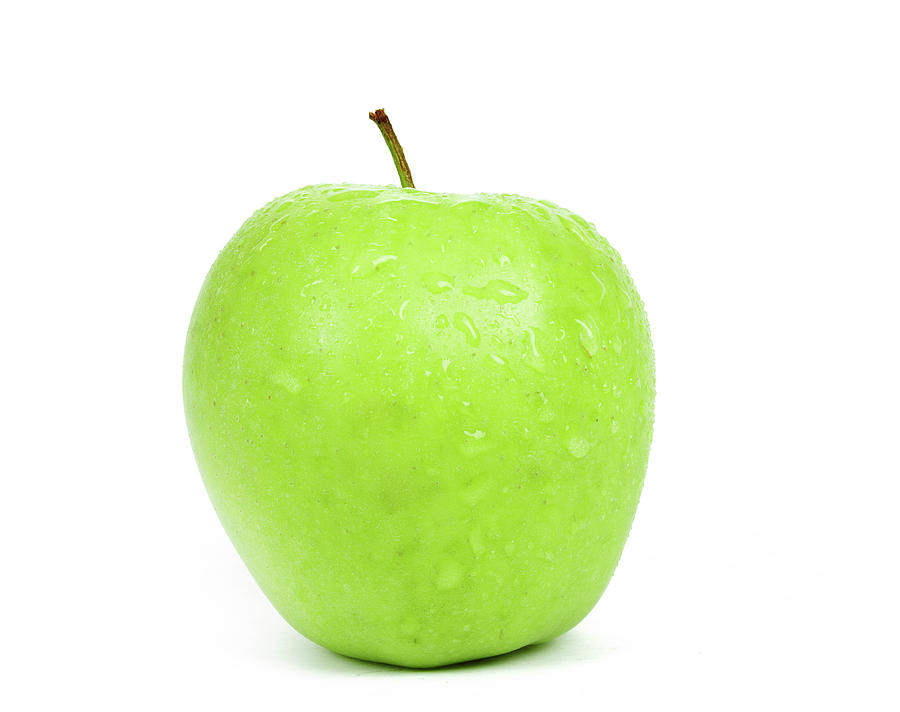
\includegraphics[width=0.48\textwidth]{images/1.jpg}\hfill
                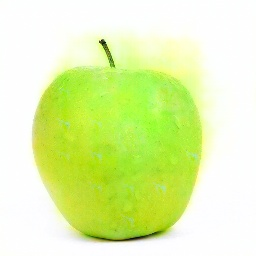
\includegraphics[width=0.48\textwidth]{images/pix2pix1.jpg}\\[1mm]
                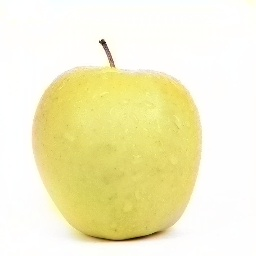
\includegraphics[width=0.48\textwidth]{images/eccv161.jpg}\hfill
                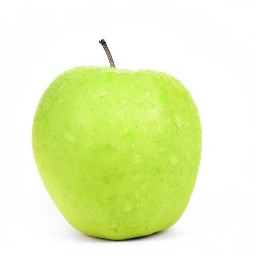
\includegraphics[width=0.48\textwidth]{images/siggraph171.jpg}\\[1mm]
                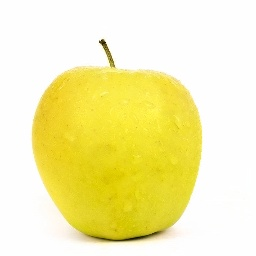
\includegraphics[width=0.48\textwidth]{images/ddcolor1.jpg}\hfill
                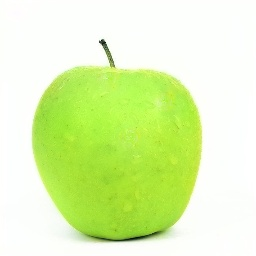
\includegraphics[width=0.48\textwidth]{images/mamba1.jpg}
                \caption{Natural Color Dataset}
            \end{subfigure}
            \hfill
            % Другий датасет (COCO 2017)
            \begin{subfigure}[t]{0.32\textwidth}
                \centering
                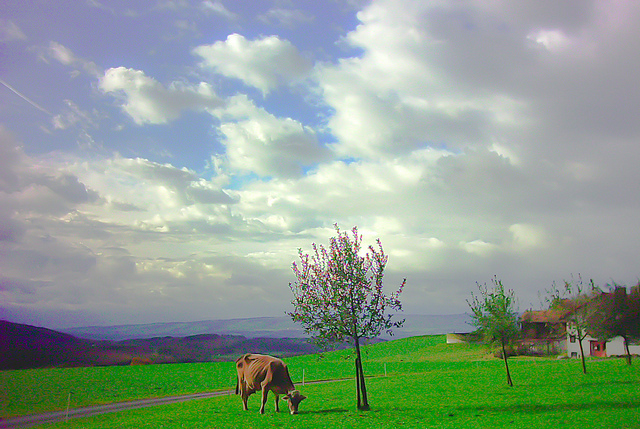
\includegraphics[width=0.48\textwidth]{images/2.jpg}\hfill
                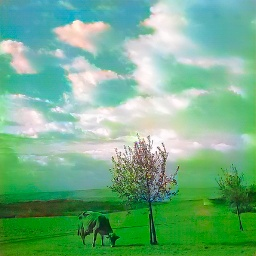
\includegraphics[width=0.48\textwidth]{images/pix2pix2.jpg}\\[1mm]
                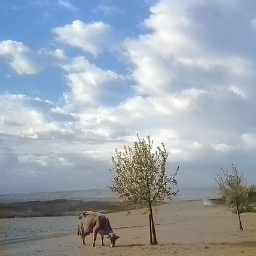
\includegraphics[width=0.48\textwidth]{images/eccv162.jpg}\hfill
                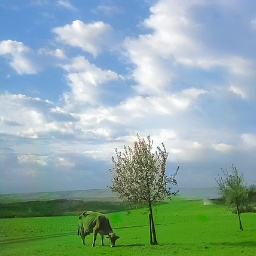
\includegraphics[width=0.48\textwidth]{images/siggraph172.jpg}\\[1mm]
                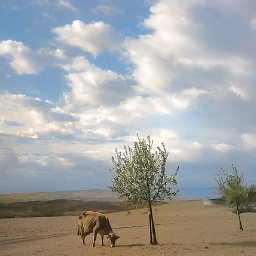
\includegraphics[width=0.48\textwidth]{images/ddcolor2.jpg}\hfill
                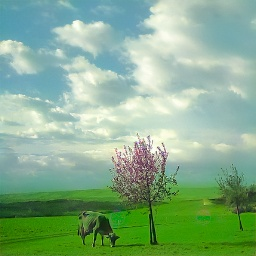
\includegraphics[width=0.48\textwidth]{images/mamba2.jpg}
                \caption{COCO 2017 Test}
            \end{subfigure}
            \hfill
            % Третій датасет (Oxford-102)
            \begin{subfigure}[t]{0.32\textwidth}
                \centering
                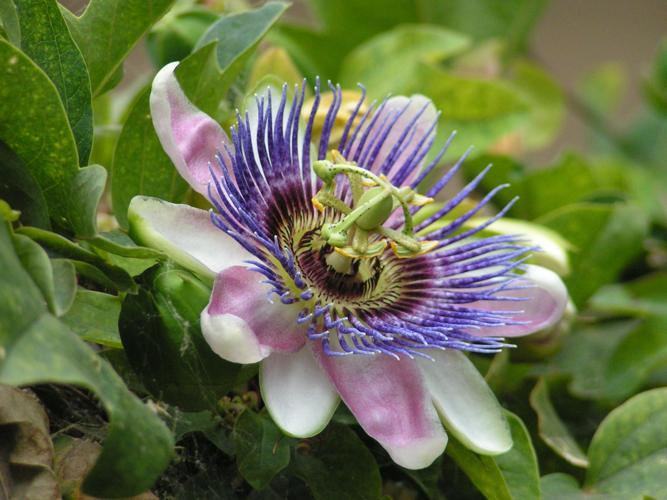
\includegraphics[width=0.48\textwidth]{images/3.jpg}\hfill
                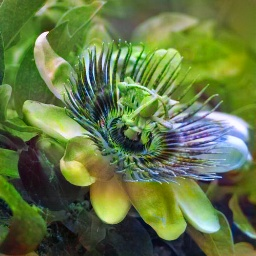
\includegraphics[width=0.48\textwidth]{images/pix2pix3.jpg}\\[1mm]
                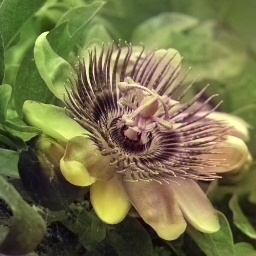
\includegraphics[width=0.48\textwidth]{images/eccv163.jpg}\hfill
                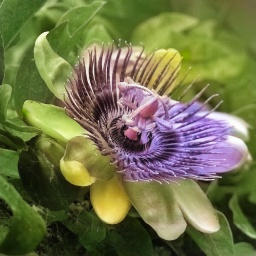
\includegraphics[width=0.48\textwidth]{images/siggraph173.jpg}\\[1mm]
                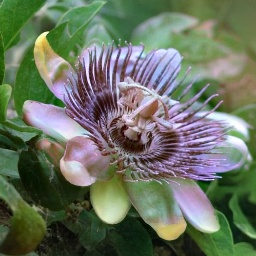
\includegraphics[width=0.48\textwidth]{images/ddcolor3.jpg}\hfill
                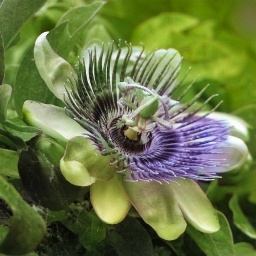
\includegraphics[width=0.48\textwidth]{images/mamba3.jpg}
                \caption{Oxford-102 Flowers}
            \end{subfigure}
            
            \caption{Візуальне порівняння результатів колоризації. У кожному блоці (зліва направо, зверху вниз): Оригінал, Pix2Pix, ECCV16, SIGGRAPH17, DDColor, B-Mamba.}
            \label{fig:visual_comparison}
        \end{figure}

        Візуальний аналіз показує, що повністю автоматична модель DDColor продемонструвала високу якість колоризації квітки (Oxford-102 Flowers).
        Проте на інших тестових зображеннях її результати виявилися менш стабільними:
        через відсутність механізму інтерактивного керування модель покладається виключно на внутрішні апріорні знання.
        У випадках візуальної невизначеності це призводить до вибору <<безпечної>>,
        тьмяної палітри -- зокрема, яблуко набуло блідого жовто-зеленого відтінку,
        а поле стало однорідно піщано-коричневим, і користувач не має інструментів для коригування цього результату.
        Натомість запропонована гібридна модель розв'язує цю проблему:
        завдяки підтримці просторових підказок вона забезпечує не лише збереження природної насиченості кольорів,
        але й дозволяє точно керувати процесом колоризації на різних типах сцен.

    \section{Користувацьке дослідження якості колоризації}
        Для всебічної оцінки візуальної якості результатів роботи запропонованої гібридної моделі
        та її порівняння з базовим методом було проведено користувацьке дослідження.
        Об'єктивні метрики не завжди корелюють із тим, як людське око сприймає реалістичність кольорів,
        тому суб'єктивна оцінка є критично важливою для задач генерації зображень.

        \subsection{Методологія проведення опитування}
            Приклад інтерфейсу етапів опитування наведено на рис.~\ref{fig:survey_interface}.
            \begin{figure}[ht!]
                \centering
                \begin{subfigure}[t]{0.32\textwidth}
                    \centering
                    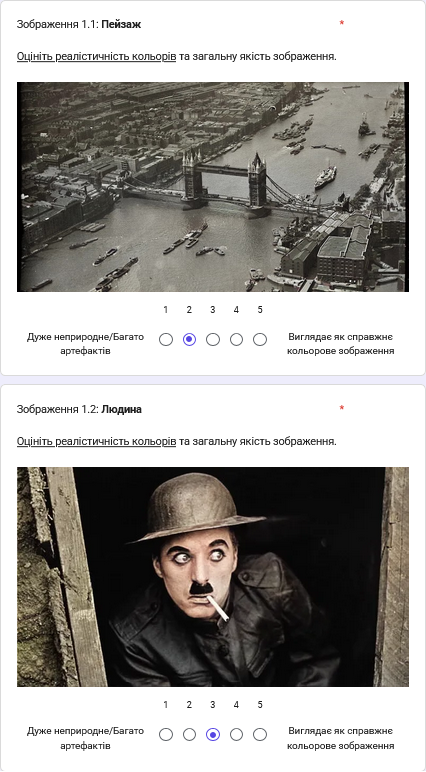
\includegraphics[width=0.9\textwidth]{images/stage1.png}
                    \caption{оцінка реалістичності}
                \end{subfigure}
                \hfill
                \begin{subfigure}[t]{0.32\textwidth}
                    \centering
                    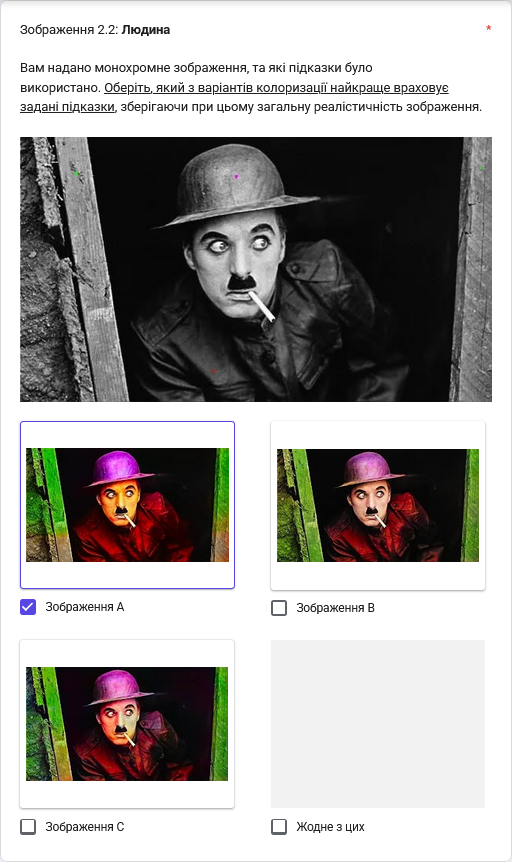
\includegraphics[width=0.9\textwidth]{images/stage2.png}
                    \caption{точність слідування підказкам}
                \end{subfigure}
                \hfill
                \begin{subfigure}[t]{0.32\textwidth}
                    \centering
                    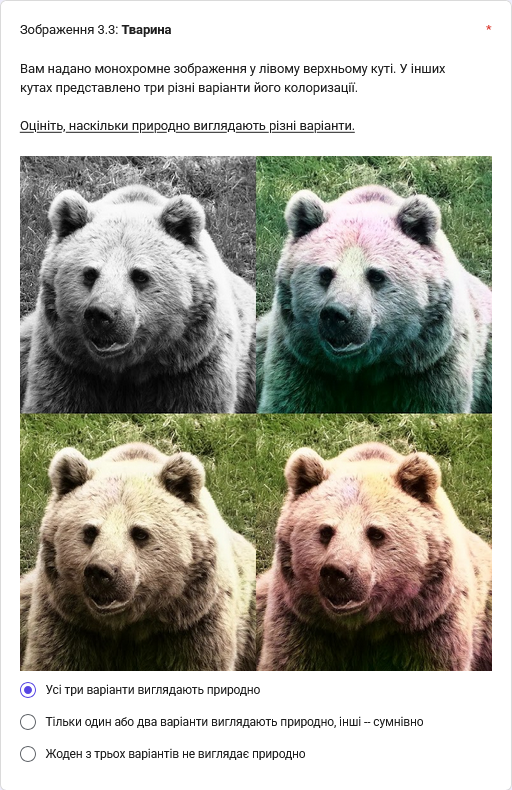
\includegraphics[width=0.9\textwidth]{images/stage3.png}
                    \caption{оцінка багатоваріантності}
                \end{subfigure}
                \caption{Інтерфейс користувацького дослідження}
                \label{fig:survey_interface}
            \end{figure}

            В опитуванні взяли участь 18 респондентів.
            Участь була повністю добровільною та анонімною, результати збиралися через платформу Google Forms.
            Для тестування було відібрано 6 категорій зображень різної складності:
            пейзаж, людина, тварина, кімната/інтер'єр, простий одиничний об'єкт та вулиця.

            Опитування складалося з ознайомлення з протоколом погодження та трьох послідовних етапів, кожен з яких був спрямований на оцінку конкретного аспекту роботи моделі:
            \begin{enumerate}
                \item протокол погодження: містить інформацію про мету дослідження, політику збору та обробки даних, а також умови використання результатів;
                \item оцінка реалістичності:
                    респондентам демонстрували колоризоване зображення
                    та пропонували оцінити його природність за 5-бальною шкалою (від 1 -- <<Дуже неприродне / Багато артефактів>> до 5 -- <<Виглядає як справжнє кольорове зображення>>);
                \item точність слідування підказкам:
                    респондентам демонстрували монохромне зображення із нанесеними колірними підказками та три варіанти колоризації від різних моделей, а саме SIGGRAPH17, Pix2Pix та нашої запропонованої моделі.
                    Завданням було обрати варіант, який найкраще враховує задані підказки, зберігаючи реалістичність;
                \item оцінка багатоваріантності: 
                    респондентам демонстрували кілька згенерованих варіантів розфарбовування одного монохромного зображення.
                    Завданням було оцінити, скільки з представлених варіантів виглядають природно.
            \end{enumerate}

        \subsection{Результати першого етапу: Оцінка реалістичності}
            На першому етапі середня оцінка реалістичності згенерованих зображень склала $3.509$ балів з $5$ можливих. Усереднені за зображеннями оцінки можна побачити на рис.~\ref{fig:chart_gen}
            \begin{figure}[ht!]
                \centering
                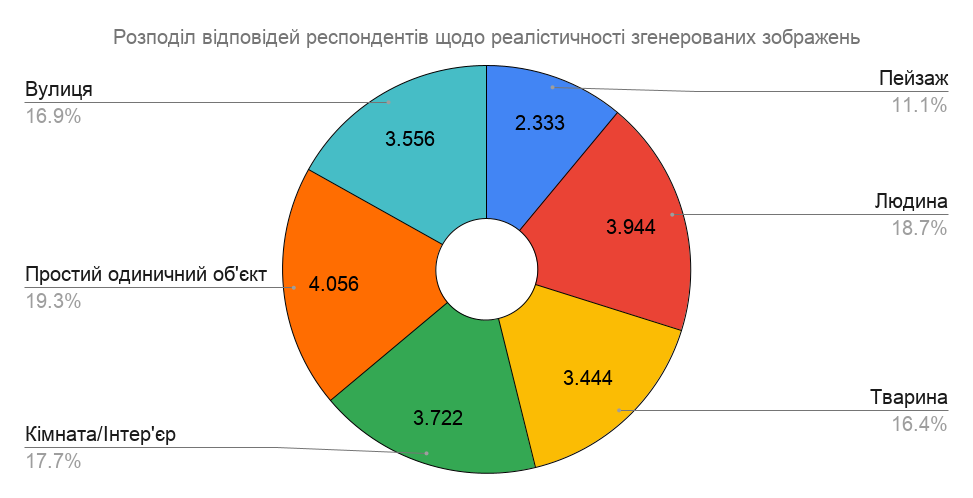
\includegraphics[width=0.75\textwidth]{images/Розподіл відповідей респондентів щодо реалістичності згенерованих зображень.png}
                \caption{Розподіл відповідей респондентів щодо реалістичності автоматично згенерованих зображень}
                \label{fig:chart_gen}
            \end{figure}
            
            Найвищі оцінки отримали зображення в категоріях <<простий одиничний об'єкт>> та <<людина>>, $4.056$ та $3.944$ бали відповідно,
            що свідчить про високу здатність моделі коректно відновлювати природні відтінки шкіри та локальні кольори ізольованих об'єктів.
            
            Зображення з великою кількістю дрібних деталей або зняті з висоти (категорії <<пейзаж>> і <<вулиця>>) отримали дещо нижчі бали, $2.333$ та $3.556$ відповідно.
            Це пояснюється складністю просторового розподілу кольору в дрібних текстурах та тяжінням моделі до безпечних сірих або сепійних відтінків у зонах із високою візуальною невизначеністю.

        \subsection{Результати другого етапу: Точність слідування підказкам}
            Цей етап мав на меті порівняти ефективність механізму інтерактивних підказок запропонованої моделі з існуючими альтернативними рішеннями (Pix2Pix та SIGGRAPH17).
            Головним критерієм оцінки була здатність нейромережі локалізувати заданий колір у межах цільового об'єкта,
            не допускаючи його неприродного розтікання на сусідні області, та водночас зберігати загальну візуальну цілісність сцени.

            Розподіл відповідей, наведений на діаграмі (рис.~\ref{fig:chart_hints}), демонструє, у яких саме категоріях зображень гібридна архітектура найкраще впоралася із завданням за оцінками респондентів. 
            \begin{figure}[ht!]
                \centering
                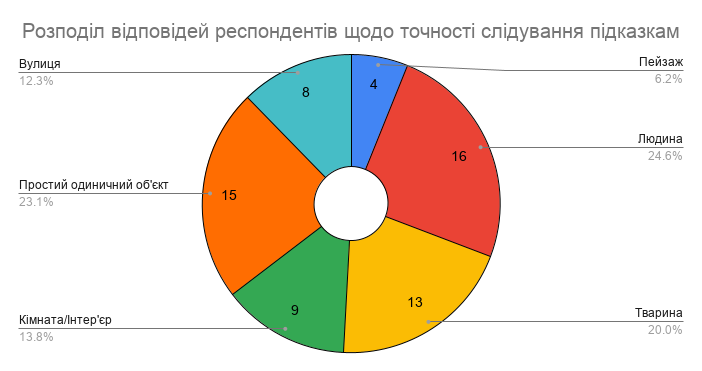
\includegraphics[width=0.75\textwidth]{images/Розподіл відповідей респондентів щодо точності слідування підказкам.png}
                \caption{Розподіл відповідей респондентів щодо точності слідування підказкам}
                \label{fig:chart_hints}
            \end{figure}
        
            Найвищі показники точності зафіксовано для категорій <<Людина>> ($16$ відповідей) та <<Простий одиничний об'єкт>> ($15$ відповідей).
            Це підтверджує ефективність інтеграції блоків B-Mamba у структуру U-Net при роботі з об'єктами, що мають чіткі семантичні межі.
            Мережа коректно реєструє просторові координати підказок і поширює заданий колір виключно в межах однорідних зон, не допускаючи ефекту <<розтікання>> на фон.
            
            Натомість найменшу кількість голосів отримала категорія <<Пейзаж>> ($4$ відповіді).
            Це пояснюється високою структурною складністю таких сцен, великою кількістю дрібних деталей, а також критичною залежністю результату від якості самих користувацьких підказок. 
            У складних ландшафтах кількох розріджених точкових маркерів виявляється недостатньо для подолання семантичної неоднозначності, що іноді призводить до ігнорування підказки або генерації артефактів.
            Це вказує на те, що для подібних зображень користувачеві необхідно надавати більш щільні та продумані колірні орієнтири.

            У $60.2\%$ випадків респонденти обрали зображення, згенероване розробленою гібридною моделлю,
            як таке, що найкраще враховує задані підказки без втрати загальної якості зображення.

        \subsection{Результати третього етапу: Оцінка багатоваріантності}
            На фінальному етапі оцінювалася здатність моделі генерувати правдоподібні альтернативні варіанти, результати можна побачити на рис.~\ref{fig:chart_multi}.
            \begin{figure}[ht!]
                \centering
                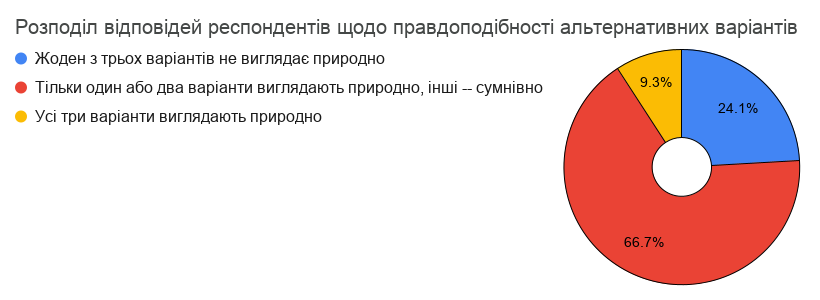
\includegraphics[width=0.75\textwidth]{images/Розподіл відповідей респондентів щодо правдоподібності альтернативних варіантів.png}
                \caption{Розподіл відповідей респондентів щодо правдоподібності альтернативних варіантів}
                \label{fig:chart_multi}
            \end{figure}
            
            У $9.3\%$ відповідей респонденти зазначили, що <<Усі три варіанти виглядають природно>>.
            У $66.7\%$ випадків користувачі обрали варіант <<Тільки один або два варіанти виглядають природно, інші -- сумнівно>>.
            
            Цей результат підтверджує, що додавання генерації випадкових підказок дозволяє створювати різні версії розфарбовування,
            але зберігати їх максимальну візуальну правдоподібність в очах людини-спостерігача буде можливо за умови,
            якщо колір для підказки генеруватиметься додатковою моделлю на основі семантики об'єкта, а не просто вибиратиметься випадковим чином із нормального розподілу.

        \subsection{Висновки за результатами користувацького дослідження}
            Проведене опитування підтвердило гіпотезу про те,
            що запропонована гібридна архітектура ефективно справляється із задачею інтерактивної багатоваріантної колоризації.
            Модель отримала високі суб'єктивні оцінки щодо загальної реалістичності,
            продемонструвала значну перевагу над базовим підходом у точності обробки локальних колірних підказок користувача,
            а також довела здатність генерувати серію альтернативних кольорових рішень для одного зображення.

\chapconclude{\ref{chap:results}}
    В ході експериментального дослідження розроблена нейромережева модель B-Mamba
    продемонструвала абсолютну перевагу над існуючими класичними аналогами ECCV16, SIGGRAPH17, Pix2Pix
    та перевершила сучасну важку архітектуру DDColor за перцептивними показниками якості генерації: FID 3.078, LPIPS 0.143.
    Водночас оптимізація через Shared Mamba дозволила скоротити використання VRAM до 187 МБ. 

    Рекордно низький $\mathrm{MSE}_{\mathrm{HINT}} = 6.1 \times 10^{-5}$ підтверджує створення бездоганно керованої інтерактивної системи,
    яка здатна в реальному часі генерувати багатоваріантні результати за бажанням користувача.

    Окрім об'єктивних метрик, результати користувацького дослідження довели високу візуальну реалістичність згенерованих зображень (середня оцінка $3.509$ з $5$ балів)
    та значну перевагу моделі в точності обробки локальних підказок (перевага у $60.2\%$ випадків порівняно з базовими методами).
    %     % Подивіться, як нераціонально використовується простір, якщо не писати 
    %     % вступи до розділів. :)

    %     % Зазвичай третій розділ присвячено опису практичного застосування або 
    %     % експериментальної перевірки аналітичних результатів, одержаних у другому 
    %     % розділі роботи. Втім, це не обов'язкова вимога, і структура основної 
    %     % частини диплому більш суттєво залежить від характеру поставлених завдань. 
    %     % Навіть якщо у вас є певне експериментальне дослідження, але його загальний 
    %     % опис займає дві сторінки, то краще приєднайте його підроздіром у 
    %     % попередній розділ.

    %     % При описі експериментальних досліджень необхідно:

    %     % \begin{itemize}
    %     % \item наводити повний опис експериментів, які проводились, параметрів 
    %     % обчислювальних середовищ, засобів програмування тощо;
    %     % \item наводити повний перелік одержаних результатів у чисельному вигляді для їх можливої 
    %     % перевірки іншими особами;
    %     % \item представляти одержані результати у вигляді таблиць та графіків, 
    %     % зрозумілих людському оку;
    %     % \item інтерпретувати одержані результати з точки зору поставленої задачі 
    %     % та загальної проблематики ваших досліджень.
    %     % \end{itemize}

    %     % У жодному разі не потрібно вставляти у даний розділ тексти 
    %     % інструментальних програм та засобів (окрім того рідкісного випадку, коли 
    %     % саме тексти програм і є результатом проведення експериментів). За 
    %     % необхідності тексти програм наводяться у додатках.


    % \chapconclude{\ref{chap:practice}}

    %     % Висновки до останнього розділу є, фактично, підсумковими під усім 
    %     % дослідженням; однак вони повинні стостуватись саме того, що розглядалось у 
    %     % розділі.